%%%%%%%%%%%%%%%%%%%%%%%%%%%%%%%%%%%%%%%%%%%%%%%%%%%%%%%%%%%%%%%%%%%%%
%                                                                   %
%                         LaTeX CV TEMPLATE                         %
%																	%
%             https://github.com/KainAber/latex-cv.git              %
%                                                                   %
%%%%%%%%%%%%%%%%%%%%%%%%%%%%%%%%%%%%%%%%%%%%%%%%%%%%%%%%%%%%%%%%%%%%%


%%%%%%%%%%%%%%%%%%%%%%%%%%% PREAMBLE %%%%%%%%%%%%%%%%%%%%%%%%%%%%%%%%

\documentclass[11pt, a4paper]{article}



% Packages

\usepackage{amssymb,mathtools,enumitem,enumerate,hyperref,xcolor}
\usepackage[english]{babel}
\usepackage[utf8]{inputenc}
\usepackage{helvet}
\usepackage{setspace}
\usepackage{ifthen}
\usepackage{tikz}


% Settings


%% Personal Info
\newcommand{\photopath}{}
\newcommand{\name}{Name}
\newcommand{\address}{}
\newcommand{\email}{}
\newcommand{\phone}{}
\newcommand{\linkedin}{}
\newcommand{\github}{}
\newcommand{\aboutme}{}
%%% Other info (competencies, skills, languages, experience, education) are edited in-line


%% Colors
%%% For 2 color mode, set rightsideaccent = leftsideaccent
%%% For 1 color mode, set leftsideaccent = 000000 and rightsideaccent = leftsidefill
\definecolor{rightsidefill}{HTML}{FFFFFF} % Fill color of right side
\definecolor{leftsidefill}{HTML}{4F9EAA} % Fill color of left side
\definecolor{leftsideaccent}{HTML}{000000} % Fill color of photo border and progress bar
\definecolor{rightsideaccent}{HTML}{4F9EAA} % Text color of headings on right side
\definecolor{rightsidetext}{HTML}{000000} % Text color on right side
\definecolor{rightsidetext2}{HTML}{888888} % Text color for dates and locations on right side
\definecolor{leftsidetext}{HTML}{FFFFFF} % Text color on left side
%%% Accent color combinations
%%% 4F9EAA 802651


%% Dimensions
\newcommand{\leftsideratio}{0.33} % Ratio of page split, 0.33 recommended
\newcommand{\margins}{1.5em} % Left / Right / Top margin on left minipage, 1.5em recommended
\newcommand{\leftsidetextpadding}{2em} % Space between photo, contact info, and separating line, change this based on number of skills etc, 3em recommended
\newcommand{\rightsidetextpadding}{3em} % Space between photo, contact info, and separating line, change this based on number of skills etc, 3em recommended
\newcommand{\photoborder}{1.5pt}


%% Fonts
\renewcommand{\familydefault}{\sfdefault} % Toggles Serif Fonts
%\usepackage{fontspec} % Toggles Helvetica and Avenir


%% Debug Mode
\newboolean{debugmode}
\setboolean{debugmode}{false} % Changes coloring to debug the geometry of minipages etc



% Other Commands


%% CV Items
%%% Creates CV Item (without bulleted descriptions)
%%%
%%% Parameters:
%%% 1. Job Title / Degree
%%% 2. Start
%%% 3. End
%%% 4. Company / School
\newcommand{\CVItem}[4]{%
\textbf{#1}\\
{\color{rightsidetext2} #2 $\cdot$ #3 $\cdot$ #4}
}


%% TikZ Progress Bar
%%% Creates progress bar of width-height ratio 10-1 colored in leftsideaccent + leftsidetext (50%)
%%%
%%% Parameters:
%%% 1. Width of progress bar
%%% 2. Percentage of progress
\newcommand{\progressbar}[2]{%
\begin{tikzpicture}
    % Background
    \fill[leftsidetext!60!leftsidefill, draw opacity=0.5, rounded corners=0.05*#1] (0,0) rectangle (#1, 0.1*#1);
    % Progress Bar
    \fill[leftsideaccent, rounded corners=0.05*#1] (0,0) rectangle (#2*#1, 0.1*#1);
    % Outline
    %\draw[leftsideaccent, rounded corners=0.05*#1] (0,0) rectangle (#1, 0.1*#1);
\end{tikzpicture}
}


%% Debug Mode Color Changes
\ifthenelse{\boolean{debugmode}}{
	\definecolor{debugcyan}{HTML}{AAEEEE}
	\definecolor{debugmagenta}{HTML}{EEAAEE}
	\definecolor{debuggreen}{HTML}{AAEEAA}
	\definecolor{debugyellow}{HTML}{EEEEAA}
}{
	\colorlet{debugcyan}{leftsidefill}
	\colorlet{debugmagenta}{leftsidefill}
	\colorlet{debuggreen}{rightsidefill}
	\colorlet{debugyellow}{rightsidefill}
}


%% Misc Settings
%%% Need not be changed
\pagestyle{empty}
\usepackage[margin=0pt]{geometry}
\setlength{\fboxsep}{0pt} % No padding around colorboxes
%\setlength{\fboxrule}{2.5pt} % Size of borders around boxes, not used currently
\setlist[itemize]{leftmargin=1em, itemsep=0pt, topsep=0pt}
\renewcommand{\labelitemi}{$\cdot$}
\setlength{\parindent}{0cm}
\frenchspacing




%%%%%%%%%%%%%%%%%%%%%%%%%% DOCUMENT %%%%%%%%%%%%%%%%%%%%%%%%%%%%%%%%%




\begin{document}

\colorbox{debugcyan}{%
\begin{minipage}[\textheight]{\leftsideratio\textwidth}
    \begin{center}
    \vspace{\margins}
    \colorbox{debugmagenta}{%
    %%%%%%%%%%%%%%%%%%%%%%%%%%%%%%%%%%%%%%%%%%%%%%%%%%%%%%%%%
    %                                                       %
    %                       LEFT SIDE                       %
    %                                                       %
    %%%%%%%%%%%%%%%%%%%%%%%%%%%%%%%%%%%%%%%%%%%%%%%%%%%%%%%%%
    \begin{minipage}[t][\textheight-\margins]{\textwidth-\margins-\margins}%
    	\color{leftsidetext}%
    	\centering%

    	\ifthenelse{\not\equal{\photopath}{}}{%
    	%%%%%%%%%%%%%%%%%%%%%%%%%%%%%%%%%%%%%%%%%%%%%%%%%%%%%%%%%
    	%                         PHOTO                         %
    	%%%%%%%%%%%%%%%%%%%%%%%%%%%%%%%%%%%%%%%%%%%%%%%%%%%%%%%%%

    	\begin{tikzpicture}[every node/.style={outer sep=0, inner sep=0}]
       		\node(img){\includegraphics[width=\textwidth-\photoborder-\photoborder, height=\textwidth-\photoborder-\photoborder]{\photopath}};
       		% Draw a circle around the picture
       		\draw[leftsideaccent, line width=\photoborder] circle [radius=0.5*\textwidth - 0.5*\photoborder];
       		% Fill the outside of the circle with a color
			\begin{scope}
    			% Clip to the area outside the circle
    			\clip (-0.5*\textwidth,-0.5*\textwidth) rectangle (3,3) (0,0) circle (0.5*\textwidth);
    			% Fill the clipped area with a color
    			\fill[leftsidefill] (-0.5*\textwidth,-0.5*\textwidth) rectangle (0.5*\textwidth,0.5*\textwidth);
			\end{scope}
    	\end{tikzpicture}
    	}{}

    	%%%%%%%%%%%%%%%%%%%%%%%%%%%%%%%%%%%%%%%%%%%%%%%%%%%%%
    	%                CONTACT DETAILS                    %
    	%%%%%%%%%%%%%%%%%%%%%%%%%%%%%%%%%%%%%%%%%%%%%%%%%%%%%

    	\ifthenelse{\not\equal{\address}{}}{%
    	\vspace{1.5em}
    	%%%%%%%%%%%%%%%%%%%
    	%     ADDRESS     %
    	%%%%%%%%%%%%%%%%%%%

    	\includegraphics[height=2em]{icons/address.png}

		\address

		}{}

		\ifthenelse{\not\equal{\email}{}}{%
		\vspace{1.5em}
		%%%%%%%%%%%%%%%%%
    	%     EMAIL     %
    	%%%%%%%%%%%%%%%%%

		\href{mailto:\email}{%
		\includegraphics[height=2em]{icons/email.png}
		}

		\href{mailto:\email}{\email}

		}{}

		\ifthenelse{\not\equal{\phone}{}}{%
		\vspace{1.5em}
		%%%%%%%%%%%%%%%%%
    	%     PHONE     %
    	%%%%%%%%%%%%%%%%%

		\includegraphics[height=2em]{icons/phone.png}

		\phone

		}{}

		\ifthenelse{\not\equal{\linkedin}{}}{%
		\vspace{1.5em}
		%%%%%%%%%%%%%%%%%%%%
    	%     LINKEDIN     %
    	%%%%%%%%%%%%%%%%%%%%

    	\href{https://www.linkedin.com\linkedin}{
		\includegraphics[height=2em]{icons/linkedin.png}
		}

		\href{https://www.linkedin.com\linkedin}{\linkedin}

		}{}

		\ifthenelse{\not\equal{\github}{}}{%
		\vspace{1.5em}
		%%%%%%%%%%%%%%%%%%
    	%     GITHUB     %
    	%%%%%%%%%%%%%%%%%%

    	\href{https://www.github.com/\github}{
		\includegraphics[height=2em]{icons/github.png}
		}

		\href{https://www.github.com/\github}{\github}

		}{}
		\vspace{\leftsidetextpadding}

	    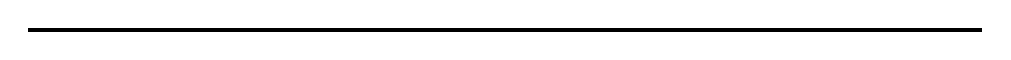
\begin{tikzpicture}
        	\draw[line cap=rect, color=leftsideaccent, line width=1.5pt] (0,0) -- (\textwidth-1.5pt,0);
    	\end{tikzpicture}

		\vspace{\leftsidetextpadding}


		%<qualities>

		%%%%%%%%%%%%%%%%%%%%%%%%%%%%%
		%     CORE COMPETENCIES     %
		%%%%%%%%%%%%%%%%%%%%%%%%%%%%%

		{\large \fontfamily{qbk}\selectfont \textbf{Core Competencies}}

		\begin{flushleft}
			\renewcommand{\arraystretch}{1.1}
			\begin{tabular}{ll}
				\progressbar{4em}{0.9} & Comp 1\\
				\progressbar{4em}{0.75} & Comp 2\\
			\end{tabular}
		\end{flushleft}

		\bigskip

		%%%%%%%%%%%%%%%%%%
		%     SKILLS     %
		%%%%%%%%%%%%%%%%%%

		{\large \fontfamily{qbk}\selectfont \textbf{Skills}}

		\begin{flushleft}
			\renewcommand{\arraystretch}{1.1}
			\begin{tabular}{ll}
				\progressbar{4em}{0.9} & Skill1\\
				\progressbar{4em}{0.75} & Skill2\\
			\end{tabular}
		\end{flushleft}

		\bigskip

		%%%%%%%%%%%%%%%%%%%%%
		%     LANGUAGES     %
		%%%%%%%%%%%%%%%%%%%%%

		{\large \fontfamily{qbk}\selectfont \textbf{Languages}}

		\begin{flushleft}
			\renewcommand{\arraystretch}{1.1}
			\begin{tabular}{ll}
				\progressbar{4em}{1} & Language 1\\
				\progressbar{4em}{0.95} & Language 2\\
			\end{tabular}
		\end{flushleft}

		%</qualities>
    \end{minipage}%
    }%
    \end{center}%
\end{minipage}%
}%
\colorbox{debugyellow}{%
\begin{minipage}[\textheight]{\textwidth-\leftsideratio\textwidth}%
    \begin{center}%
    \vspace{\margins}%
    \colorbox{debuggreen}{%
    \color{rightsidetext}
    %%%%%%%%%%%%%%%%%%%%%%%%%%%%%%%%%%%%%%%%%%%%%%%%%%%%%%%%%
    %                                                       %
    %                      RIGHT SIDE                       %
    %                                                       %
    %%%%%%%%%%%%%%%%%%%%%%%%%%%%%%%%%%%%%%%%%%%%%%%%%%%%%%%%%
    \begin{minipage}[t][\textheight-\margins]{0.9\textwidth}%
    	\vspace{\margins}%
   		%%%%%%%%%%%%%%%%%%%%%%%%%%%%%%%%%%%%%%%%%%%%%%%%%%%%%%%%%
   	 	%                HEADLINE & ABOUT ME                    %
    	%%%%%%%%%%%%%%%%%%%%%%%%%%%%%%%%%%%%%%%%%%%%%%%%%%%%%%%%%
    	\begin{flushleft}%
    		{\Huge \color{rightsideaccent} \fontfamily{qbk}\selectfont \textbf{\name}}
    	\end{flushleft}

    	\ifthenelse{\not\equal{\phone}{}}{%

    	\bigskip

    	\textit{\aboutme}
    	}{}

    	\vspace{\rightsidetextpadding}

        %<vita>

    	%%%%%%%%%%%%%%%%%%%%%%
		%     EXPERIENCE     %
		%%%%%%%%%%%%%%%%%%%%%%
    	{\LARGE \color{rightsideaccent} \fontfamily{qbk}\selectfont \textbf{Experience}}

    	\bigskip

		\CVItem{Job Title}{from}{to}{Company}

		\begin{itemize}
 			\item item1
 			\item item2
 			\item item3
 		\end{itemize}

    	\vspace{\rightsidetextpadding}

    	%%%%%%%%%%%%%%%%%%%%%%
		%     EXPERIENCE     %
		%%%%%%%%%%%%%%%%%%%%%%

    	{\LARGE \color{rightsideaccent} \fontfamily{qbk}\selectfont \textbf{Education}}

		\bigskip

		\CVItem{Title}{From}{to}{Institution}\\

		%</vita>
    \end{minipage}
    }
    \end{center}
\end{minipage}
}

\end{document}
